\section{User management}
\label{sec:USR_user_management}

Le app rivolte ad una comunità di utenti/clienti devono necessariamente implementare i meccanismi di gestione dell'utente.

I meccanismi di gestione utente base sono:
\begin{itemize}
\item login dell'utente
\item signup dell'utente
\item ogout dell'utente
\item gestione del profilo utente
\end{itemize}

A questi, possono essere associati meccanismi di gestione avanzati, quali:
\begin{itemize}
\item meccanismo di verifica email
\item meccanismo di cambio email
\item meccanismo di recovery/reset password
\item meccanismo di cambio password
\end{itemize}

I meccanismi di gestione avanzata, che prevedono l'uso della mail, devono necessariamente basarsi su un servizio di gestione della mail.
Sfida del presente progetto, è riuscire ad incapsulare tali meccanismi/comportamenti in relativi elementi, per permettere così di integrare la gestione dell'utente con la stessa semplicità con cui si inseriscono elementi HTML in una pagina.


\subsection{User Management services}
\label{subsec:USR_user_management_services}
In questa sezione si parla dei vari servizi esistenti per la gestione dell'utente come: Stormpat, Userapp e Auth0.

\subsubsection{Stormpath}

Stormpath is a User Management API that reduces development time with instant-on, scalable user infrastructure. Stormpath's intuitive API and expert support make it easy for developers to authenticate, manage and secure users and roles in any application.

At Stormpath, we have a simple goal: give developers a complete user management system, so you can focus on building great applications.

\begin{itemize}
\item Pre-built authentication \& authorization.
\item Schemaless, secure user data \& profiles.
\item Code-free Active Directory, Facebook \& Google login.
\item Open Source SDKs \& complete sample apps.
\end{itemize}

\begin {figure}[h]
\graphicspath{{images/chapter_USR/}}
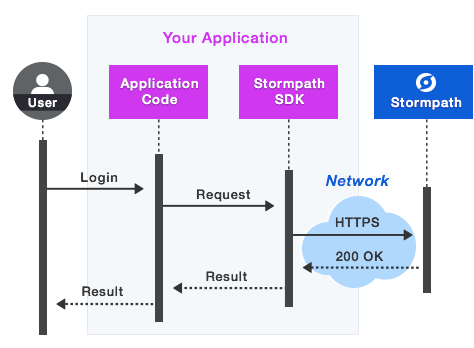
\includegraphics[width=\textwidth]{stormpath}
\caption{Stormpath User Management API}
\end {figure}

\subsubsection{Userapp}



- auth0

https://stormpath.com/

https://www.userapp.io/

https://auth0.com


\subsection{User Management API in StrongLoop LoopBack}

x-project is based on StrongLoop LoopBack on the server side.
LoopBack provides User Management.


Per la gestione della email, LoopBack si può connettere a vari providers.

Nello specifico, è stato implementata la connessione con il servizio di MailChimp chiamato Mandrill (vedi sezione...)
